\documentclass{standalone}
\usepackage{pgfplots}
\pgfplotsset{compat=1.18}
\usepgfplotslibrary{colorbrewer}
\pgfplotsset{cycle list/Set1-6}

\begin{document}

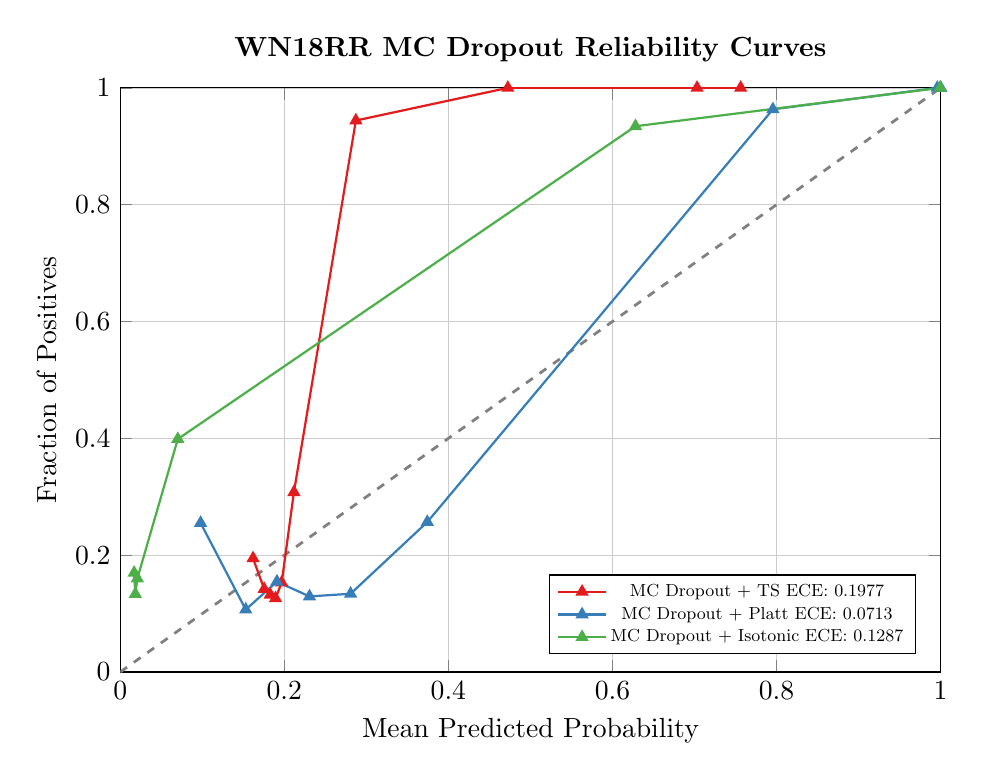
\begin{tikzpicture}
\begin{axis}[
    title={\textbf{WN18RR MC Dropout Reliability Curves}},
    xlabel={Mean Predicted Probability},
    ylabel={Fraction of Positives},
    xmin=0, xmax=1,
    ymin=0, ymax=1,
    xtick={0, 0.2, 0.4, 0.6, 0.8, 1.0},
    ytick={0, 0.2, 0.4, 0.6, 0.8, 1.0},
    legend pos= south east,
    legend style={nodes={scale=0.7, transform shape}, font=\small},
    grid=both,
    grid style={line width=.1pt, draw=gray!20},
    major grid style={line width=.2pt, draw=gray!40},
    width=12cm,
    height=9cm,
    cycle list name=Set1-6
]

% Perfectly Calibrated Line
\addplot [color=gray, dashed, line width=1pt, forget plot]
    coordinates {(0,0)(1,1)};


\addplot+[mark=triangle*, thick] coordinates { (0.16189039, 0.19457735) (0.17546051, 0.14194577) (0.18287130, 0.13237640) (0.18930686, 0.12619808) (0.19677480, 0.15311005) (0.21169342, 0.30781499) (0.28721173, 0.94408946) (0.47246310, 1.00000000) (0.70312737, 1.00000000) (0.75629165, 1.00000000) };
\addlegendentry{MC Dropout + TS ECE: 0.1977}


\addplot+[mark=triangle*, thick] coordinates { (0.09794879, 0.25518341) (0.15294447, 0.10685805) (0.19095480, 0.15470494) (0.23068458, 0.12939297) (0.28079626, 0.13397129) (0.37429243, 0.25677831) (0.79555893, 0.96325879) (0.99598420, 1.00000000) (0.99999286, 1.00000000) (0.99999935, 1.00000000) };
 \addlegendentry{MC Dropout + Platt ECE: 0.0713}

\addplot+[mark=triangle*, thick] coordinates { (0.01693974, 0.16983305) (0.01837741, 0.13352827) (0.02084091, 0.16007194) (0.07016192, 0.39878543) (0.62805058, 0.93434343) (0.99945111, 1.00000000) }; 
\addlegendentry{MC Dropout + Isotonic ECE: 0.1287}


\end{axis}
\end{tikzpicture}

\end{document}